% This document should list all the parts for the device
\section{Parts List}

\subsection{Part quantities}

\begin{tabular}{|l|c|}
    \hline
    \textbf{Part} & \textbf{Qty.}\\
    \hline
    \hyperlink{esp32}{SparkFun ESP32 Thing} & 1\\
    \hline
    \hyperlink{light}{Photoresistor GM5539} & 1\\
    \hline
    \hyperlink{temp}{Temperature Sensor} & 3\\
    \hline
    \hyperlink{salinity}{Water Sensor} & 1\\
    \hline
    \hyperlink{turbidity}{Turbidity Sensor} & 1\\
    \hline
    \hyperlink{nalgene}{Nalgene Bottle} & 1\\
    \hline
    \hyperlink{cable}{2-ft. Waterproof cable} & 1\\
    \hline
    \hyperlink{cable}{6-ft. Waterproof cable} & 1\\
    \hline
    \hyperlink{minibread}{Mini Breadboard} & 2\\
    \hline
    \hyperlink{jumperwires}{M-to-M jumper wires} & 2\\
    \hline
    \hyperlink{jumperwires}{M-to-F jumper wires} & 14\\
    \hline
    \hyperlink{jumperwires}{F-to-F jumper wires} & 2\\
    \hline
    \hyperlink{batteryholder}{2-AA battery holder} & 1\\
    \hline
    \hyperlink{battery}{AA battery} & 2\\
    \hline
    \hyperlink{silica}{Silica gel packet} & 2\\
    \hline
    \hyperlink{glue}{Silicone glue} & 1\\
    \hline

\end{tabular}

% Each subsection is a category of parts
\subsection{System on a chip (SoC)}

% first, name of item
\hypertarget{esp32}{}
\subsubsection{SparkFun ESP32 Thing}

% second, image
\hspace{2em}
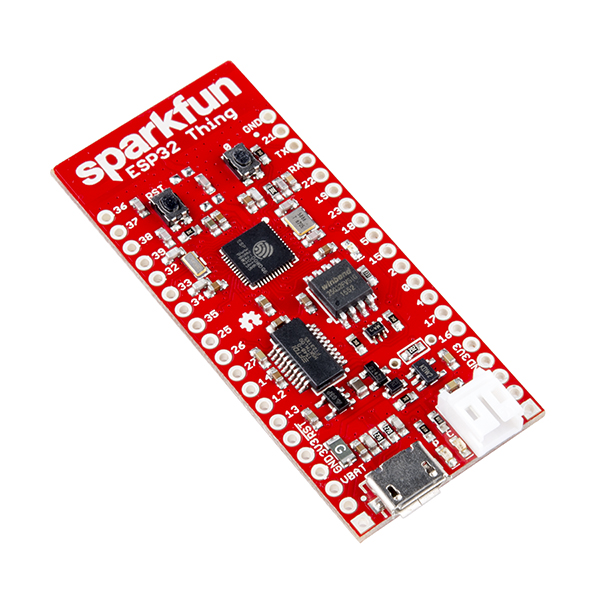
\includegraphics[scale=1.0]{esp32Soc.jpg}

\begin{flushleft}
% third, short description
    The main processing unit is a SparkFun ESP32 Thing development board from 
    Espressif. This SoC has Wi-Fi, Bluetooth 4.0, and BLE capabilities, which 
    are necessary for our system.
    \newline

    % fourth, store link
    Online store link: \newline
    \footnotesize\url{https://www.sparkfun.com/products/13907}

    % fifth, data-sheet link
    \normalsize Datasheet link: \newline
    \footnotesize\url{https://cdn.sparkfun.com/datasheets/IoT/esp32_datasheet_en.pdf}
\end{flushleft}

\subsection{Sensors}

\hypertarget{light}{}
\subsubsection{Photoresistor GM5539}

\hspace{2em}
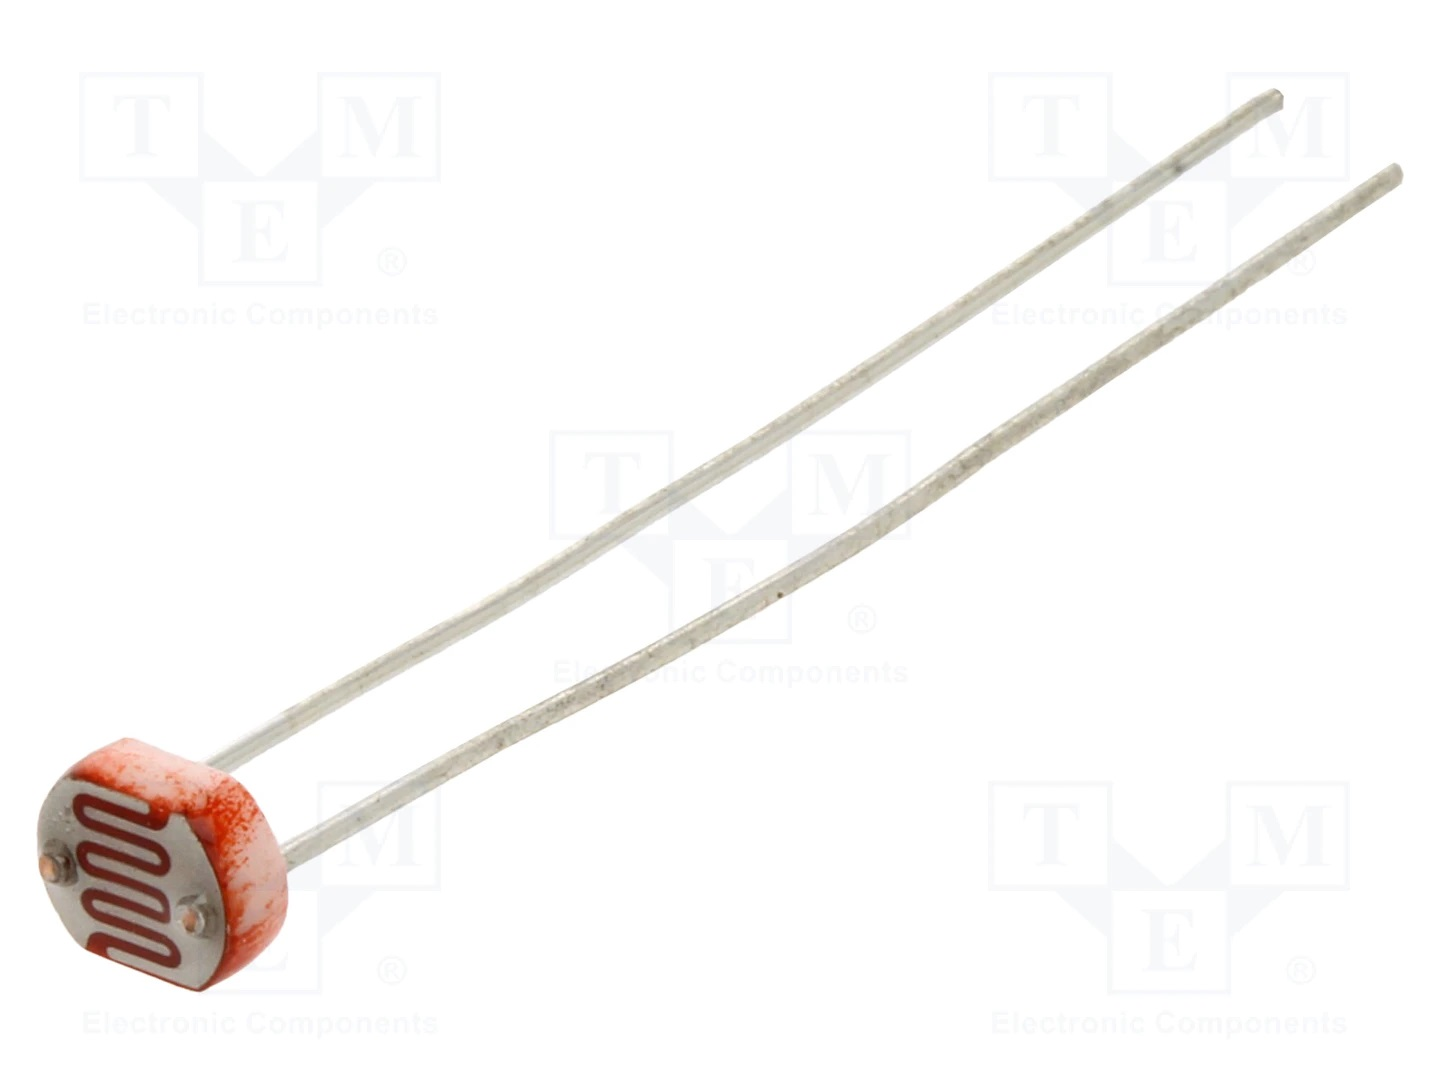
\includegraphics[scale=0.15]{photoresistor.jpg}

\begin{flushleft}
    The GM5539 Photoresistor is used to measure the amount of light hitting the
     sensor.
    \newline

    Online store link: \newline
    \footnotesize\url{https://www.amazon.com/goeasybuy-Sensitive-Resistor-Photoresistor-Optoresistor/dp/B01CGCNO34}

    \normalsize Datasheet link: \newline
    \footnotesize\url{https://www.tme.eu/Document/01ba1573cea1124ddd9a55cccc53ed63/all.pdf}
\end{flushleft}

\hypertarget{temp}{}
\subsubsection{Temperature Sensor}

\hspace{2em}
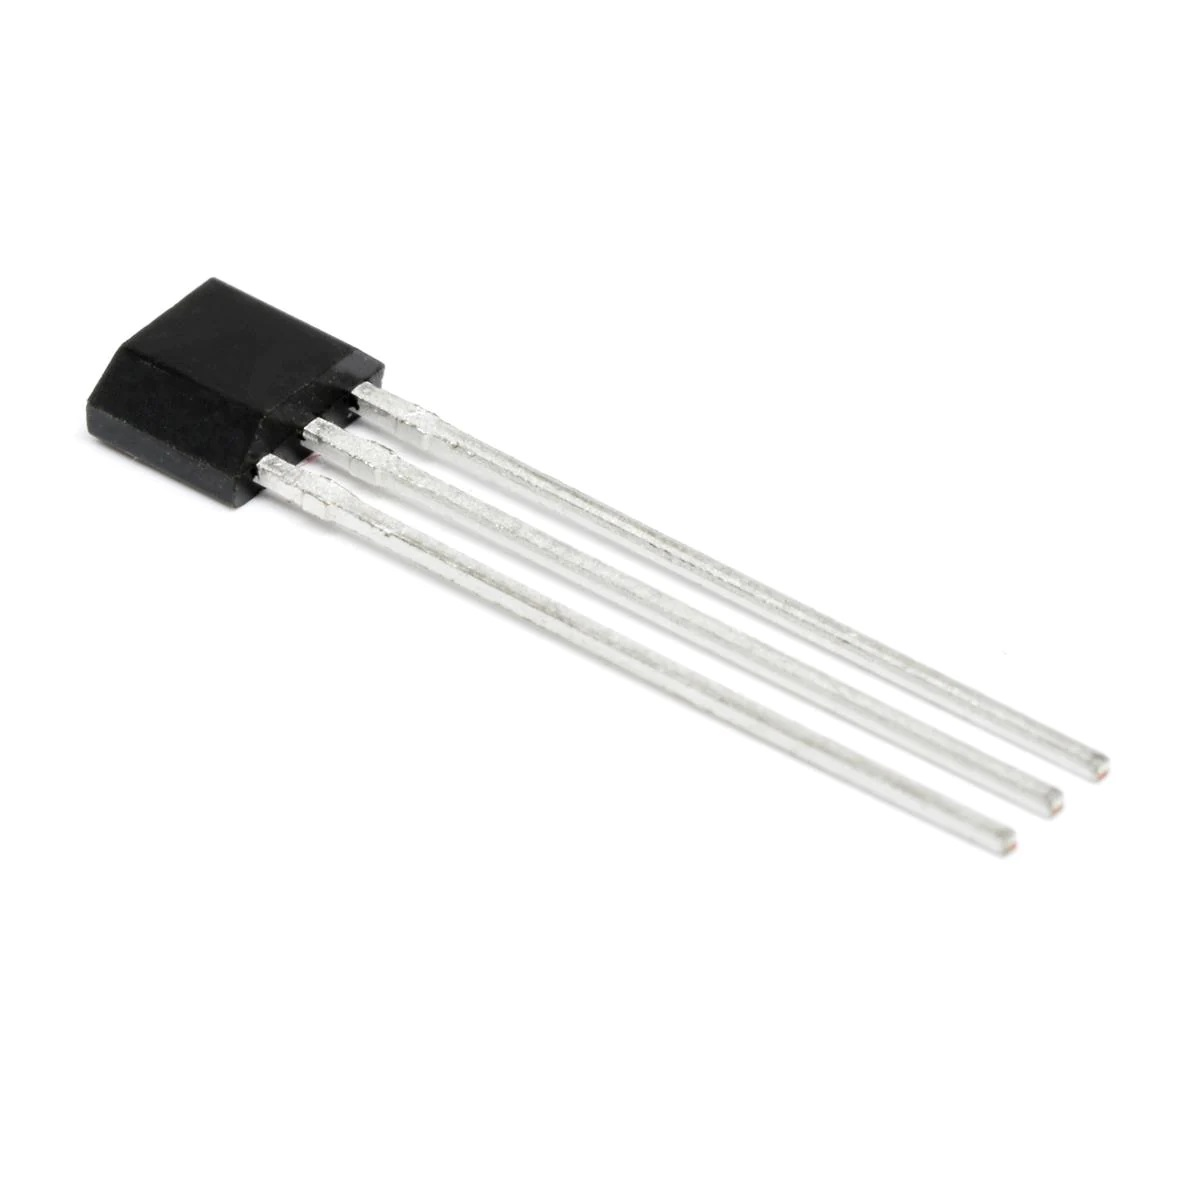
\includegraphics[scale=0.15]{tempsensor.jpg}

\begin{flushleft}
    The TMP36GT9Z temperature sensor from Analog Devices is used to measure 
    the temperature inside the nalgene bottle (at the surface level), 
    immediately underneath the water by the nalgene bottle, and 6 feet deep in 
    the water.
    \newline

    Online store link: \newline
    \footnotesize\url{https://www.mouser.com/ProductDetail/Analog-Devices/TMP36GT9Z?qs=sGAEpiMZZMv9Q1JI0Mo%2FtZYNPIqRJ81F}

    \normalsize Datasheet link: \newline
    \footnotesize\url{https://www.mouser.com/datasheet/2/609/TMP35_36_37-1504323.pdf}
\end{flushleft}

\hypertarget{salinity}{}
\subsubsection{Water Sensor}

\hspace{2em}
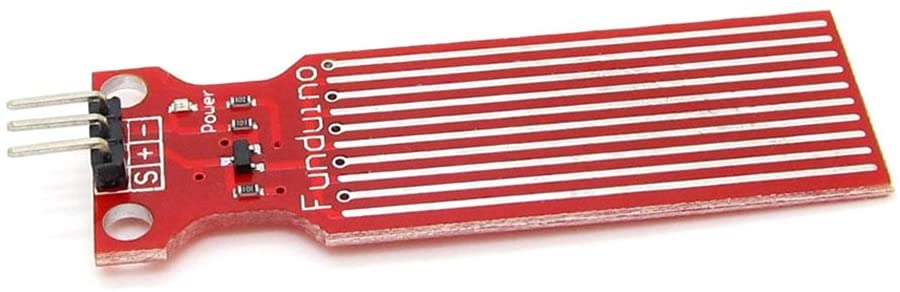
\includegraphics[scale=0.2]{watersensor.jpg}

\begin{flushleft}
    The water sensor is to detect the salinity of the water. Purely diststilled
     water will not be detected, but the contacts will corrode more as it stays
     longer in the water with the more salinity in the water. The more salinity
     that is in contact, the more energy is flowed through the contacts.
    \newline

    Online store link: \newline
    \footnotesize\url{https://www.amazon.com/Sensor-module-Detection-Surface-Arduino/dp/B01N058HS6/}

    \normalsize Datasheet link: \newline
    \footnotesize \emph{N/A}
\end{flushleft}

\hypertarget{turbidity}{}
\subsubsection{Turbidity Sensor}

\hspace{2em}
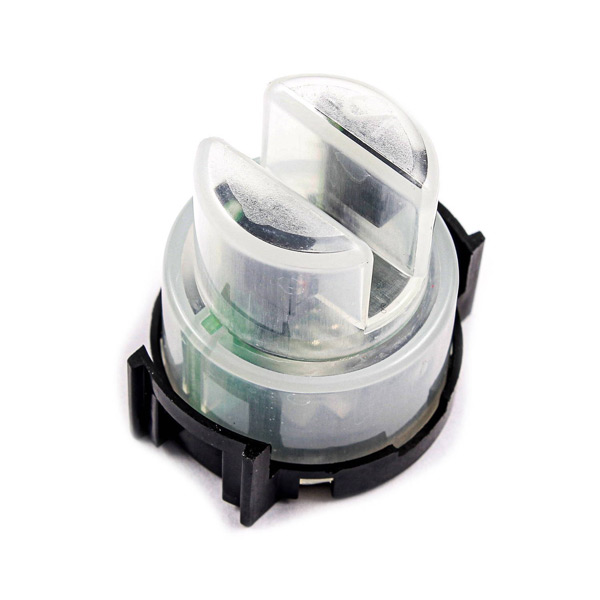
\includegraphics[scale=0.15]{turbidity.jpg}

\begin{flushleft}
    The TSD-10 turbidity sensor from Amphenol Advanced Sensors is to measure 
    the amount of light being received from the output source to the sensor.
    \newline

    Online store link: \newline
    \footnotesize\url{https://www.newark.com/amphenoladvanced-sensors/tsd-10/turbidity-sensor-5vdc-phototransistor/dp/18X9859}

    \normalsize Datasheet link: \newline
    \footnotesize\url{http://www.farnell.com/datasheets/1855958.pdf}
\end{flushleft}

\subsection{Prototyping/Development}

\subsubsection{Breadboard}

\hspace{2em}
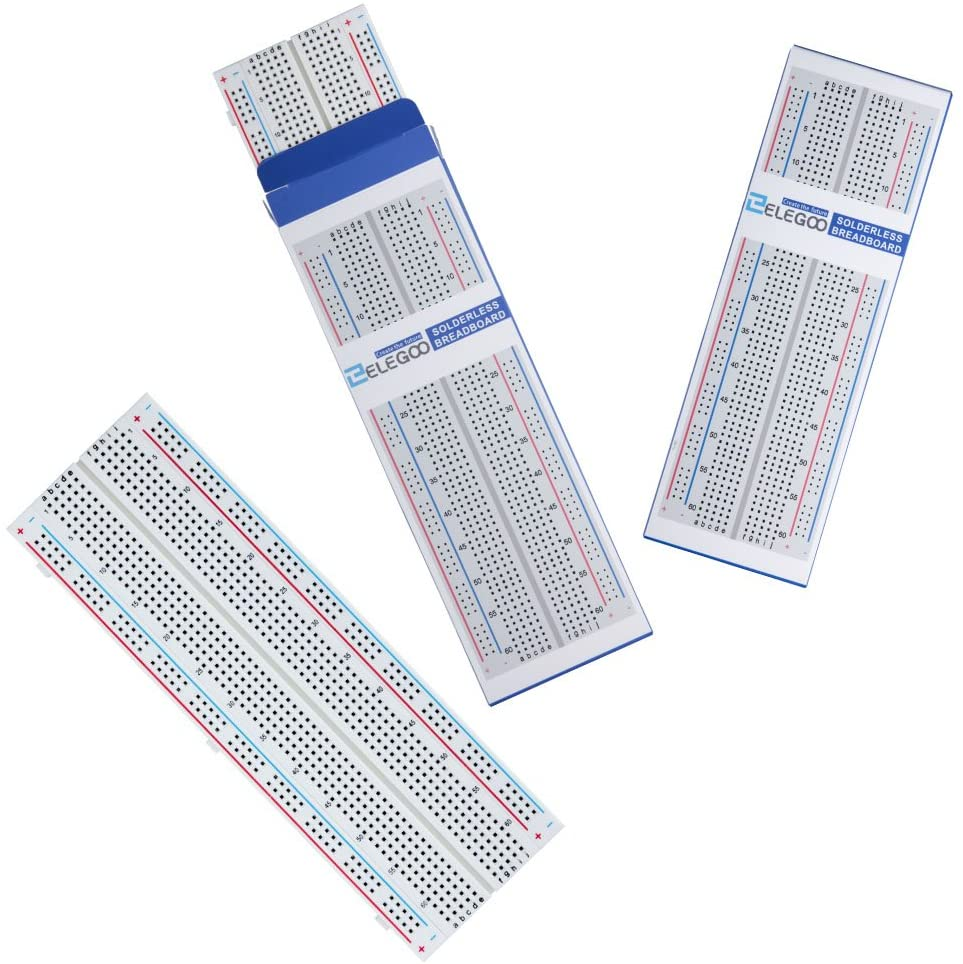
\includegraphics[scale=0.1]{breadboard.jpg}

\begin{flushleft}
    A simple yet useful platform to easily design and prototype circuits for 
    the hardware buoy. Keeps everything attached to one platform, like the 
    sensors, SoC, and wiring.
    \newline

    Online store link: \newline
    \footnotesize\url{https://www.amazon.com/EL-CP-003-Breadboard-Solderless-Distribution-Connecting/dp/B01EV6LJ7G}

\end{flushleft}

\subsubsection{Breadboard wires}

\hspace{2em}
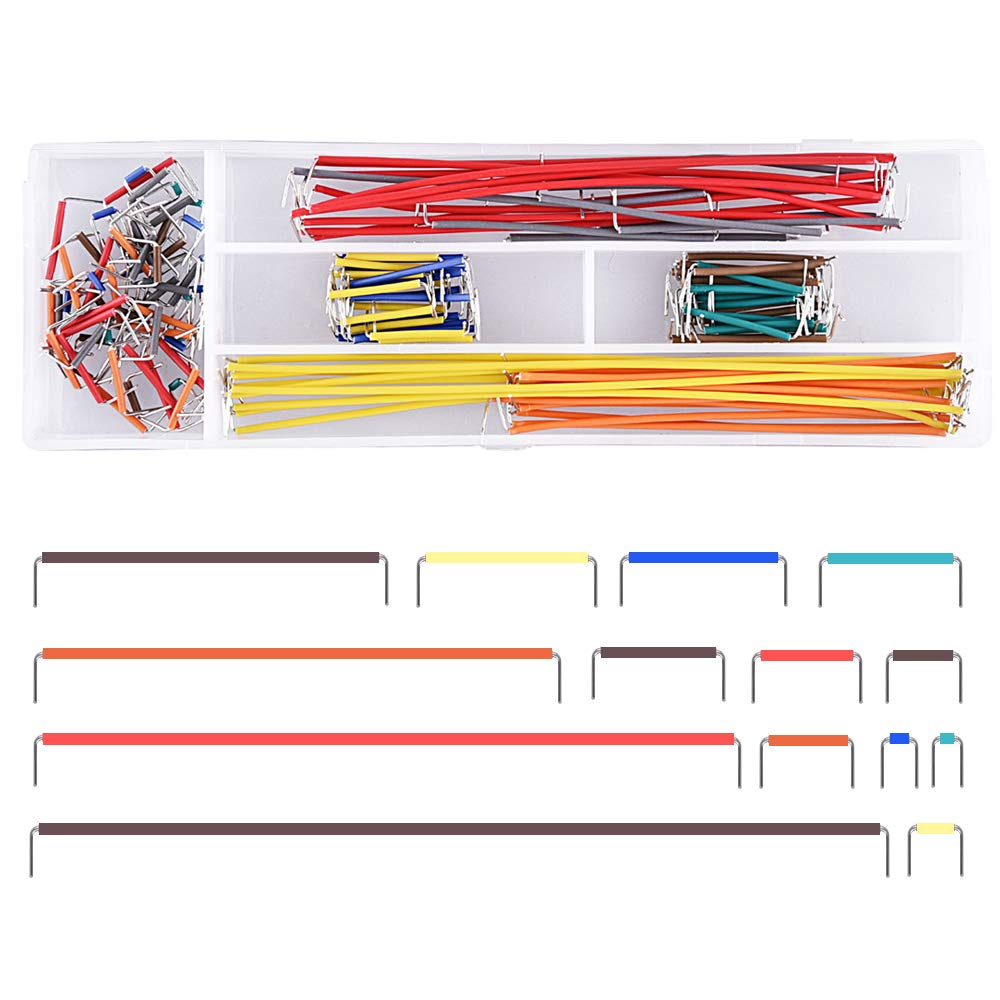
\includegraphics[scale=0.07]{breadboardwires.jpg}

\begin{flushleft}
    Layout the circuit with various sized wires to make a clean and modifiable 
    design for the hardware buoy.
    \newline

    Online store link: \newline
    \footnotesize\url{https://www.amazon.com/AUSTOR-Preformed-Breadboard-Assorted-Prototyping/dp/B07PQKNQ22}

\end{flushleft}

\subsection{Production Buoy}

\hypertarget{nalgene}{}
\subsubsection{Nalgene Bottle}

\hspace{2em}
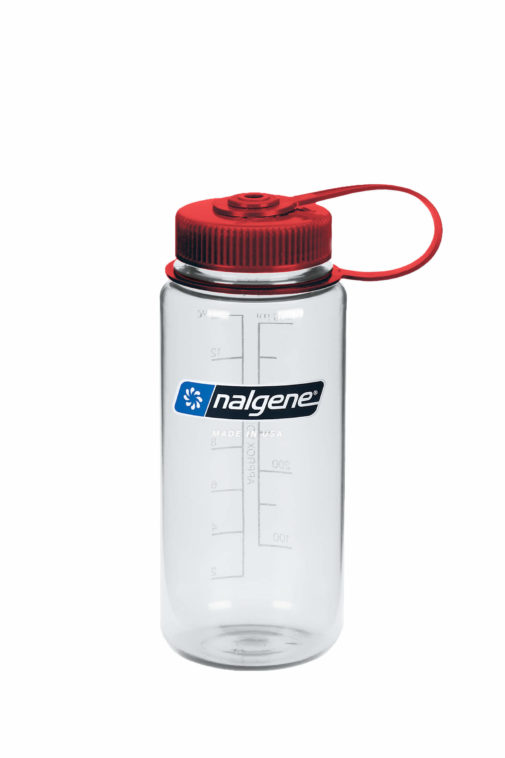
\includegraphics[scale=0.12]{nalgene.jpg}

\begin{flushleft}
    16 oz. Nalgene bottle featuring a screw-top lid for the mouth opening. 
    This is the vessel for our hardware, which will live inside the bottle 
    with 2 outlets (holes) that will be made in the lid to lead out sensors 
    out to 2 feet and 6 feet underneath the water.
    \newline

    Online store link: \newline
    \footnotesize\url{https://nalgene.com/product/16oz-wide-mouth-bottle/?attribute_pa_color=clear}

\end{flushleft}

\hypertarget{cable}{}
\subsubsection{Waterproof cable}

\hspace{2em}
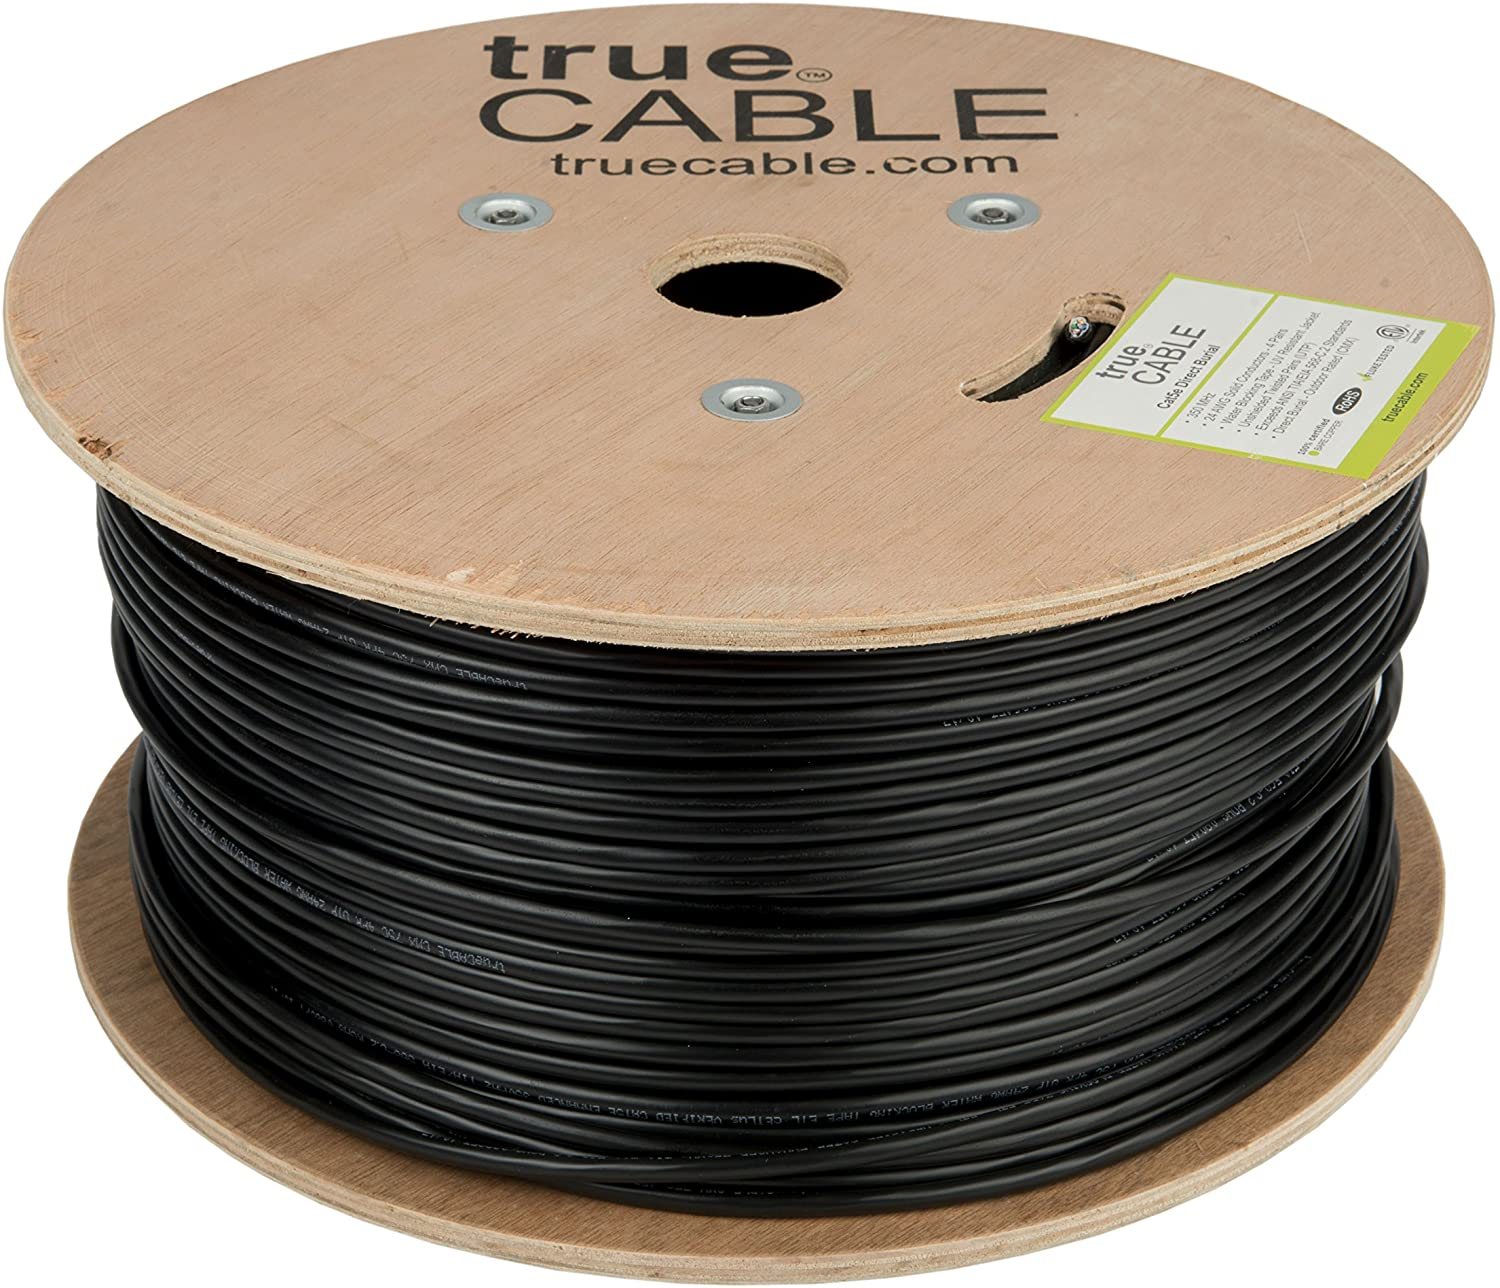
\includegraphics[scale=0.08]{ethernetcable.jpg}

\begin{flushleft}
    This Cat5e cable has a waterproof rating, which is perfect for our 
    application. There are many leads available to wire up all the sensors to 
    the ESP32. This cord will be cut into a 2-foot piece and a 6-foot piece.
    It comes in a 500-foot roll.
    \newline

    Online store link: \newline
    \footnotesize\url{https://www.amazon.com/dp/B01JAVNK2E}

\end{flushleft}

\hypertarget{minibread}{}
\subsubsection{Mini Breadboard}

\hspace{2em}
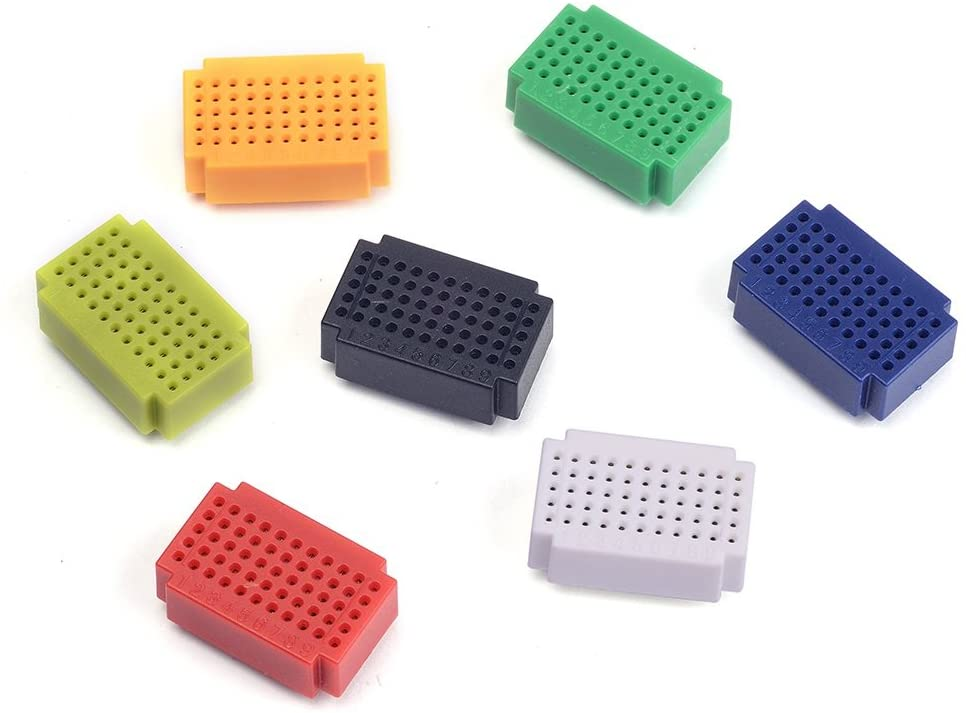
\includegraphics[scale=0.1]{minibreadboard.jpg}

\begin{flushleft}
    Smaller, more managable breadboard in a tight volume of the nalgene bottle 
    will help keep all the wiring together and provide power for all sensors.
    \newline

    Online store link: \newline
    \footnotesize\url{https://www.amazon.com/Cylewet-Solderless-Circuit-Arduino-CYT1030/dp/B01N9MIH1T}

\end{flushleft}

\hypertarget{jumperwires}{}
\subsubsection{Jumper wires}

\hspace{2em}
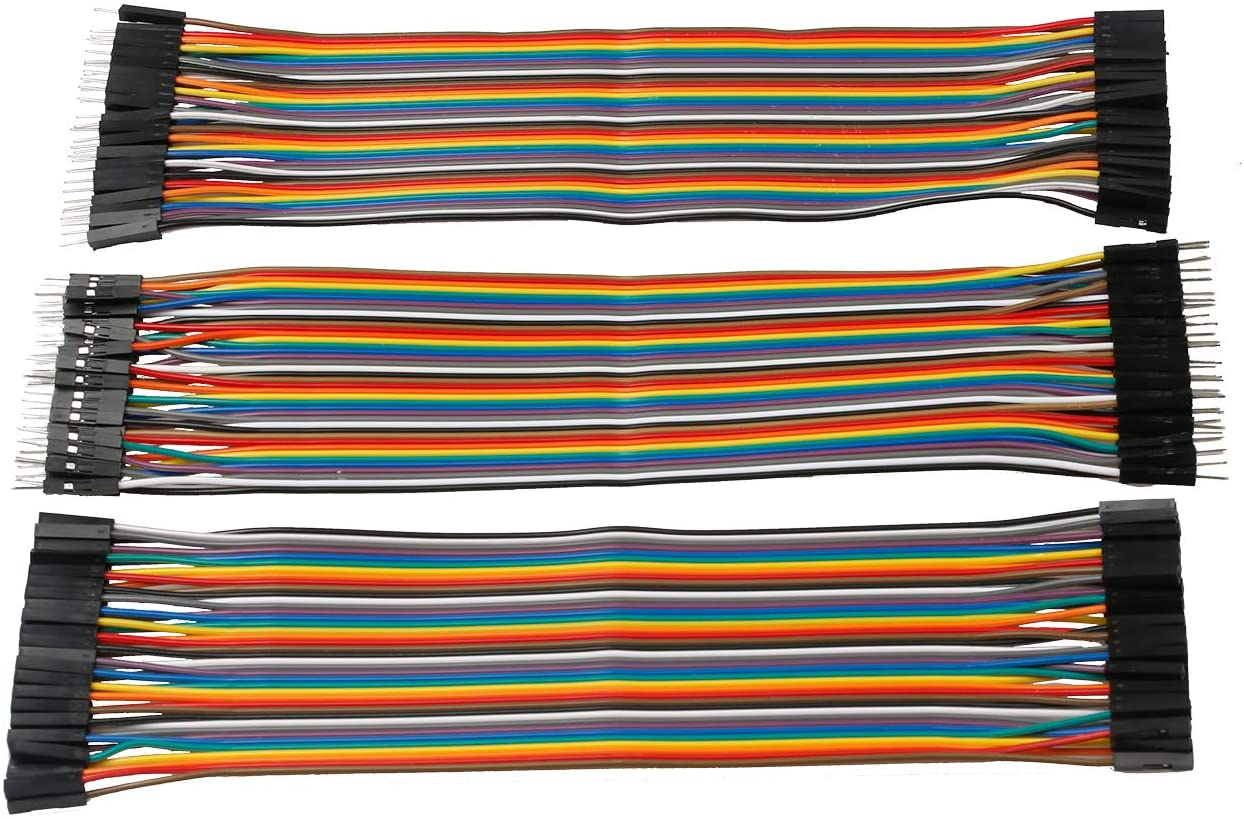
\includegraphics[scale=0.1]{jumperwires.jpg}

\begin{flushleft}
    A set of Male-to-Male, Male-to-Female, and Female-to-Female breadboard 
    jumper wires for connecting the photoresistor, temperature, and ESP32 pins 
    together to the breadboards. Each buoy only needs about 12 wires, but the 
    linked set of jumper wires offers the best price.
    \newline

    Online store link: \newline
    \footnotesize\url{https://www.amazon.com/EDGELEC-Breadboard-Optional-Assorted-Multicolored/dp/B07GD2BWPY/}

\end{flushleft}

\hypertarget{batteryholder}{}
\subsubsection{2-AA battery holder}

\hspace{2em}
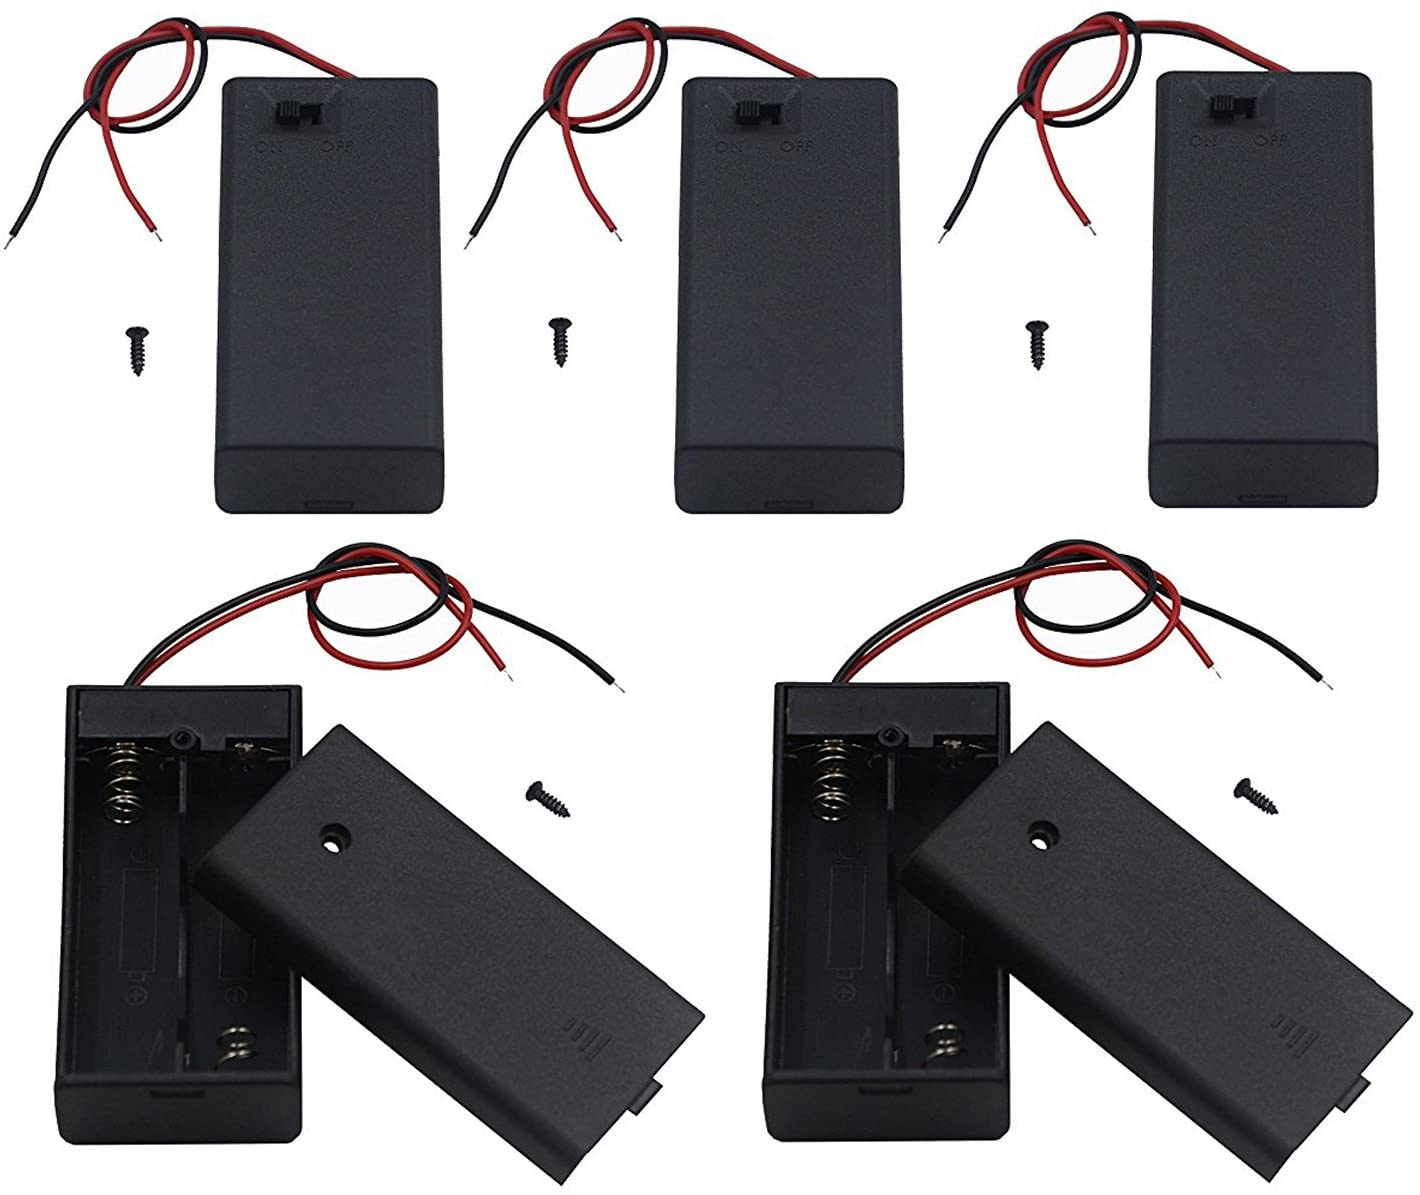
\includegraphics[scale=0.1]{batteryholder.jpg}

\begin{flushleft}
    An AA battery holder with positive and negative lead wires and a 
    power switch.
    \newline

    Online store link: \newline
    \footnotesize\url{https://www.amazon.com/dp/B076C7S2VN/}

\end{flushleft}

\hypertarget{battery}{}
\subsubsection{AA batteries}

\hspace{2em}

\includegraphics[scale=0.1]{aabatteries.jpg}

\begin{flushleft}
    A typical set of AA batteries by Duracell at 1.5 volts.
    \newline

    Online store link: \newline
    \footnotesize\url{https://www.amazon.com/Duracell-CopperTop-Batteries-all-purpose-household/dp/B003SI0TD4}

\end{flushleft}

\hypertarget{silica}{}
\subsubsection{Silica Gel}

\hspace{2em}
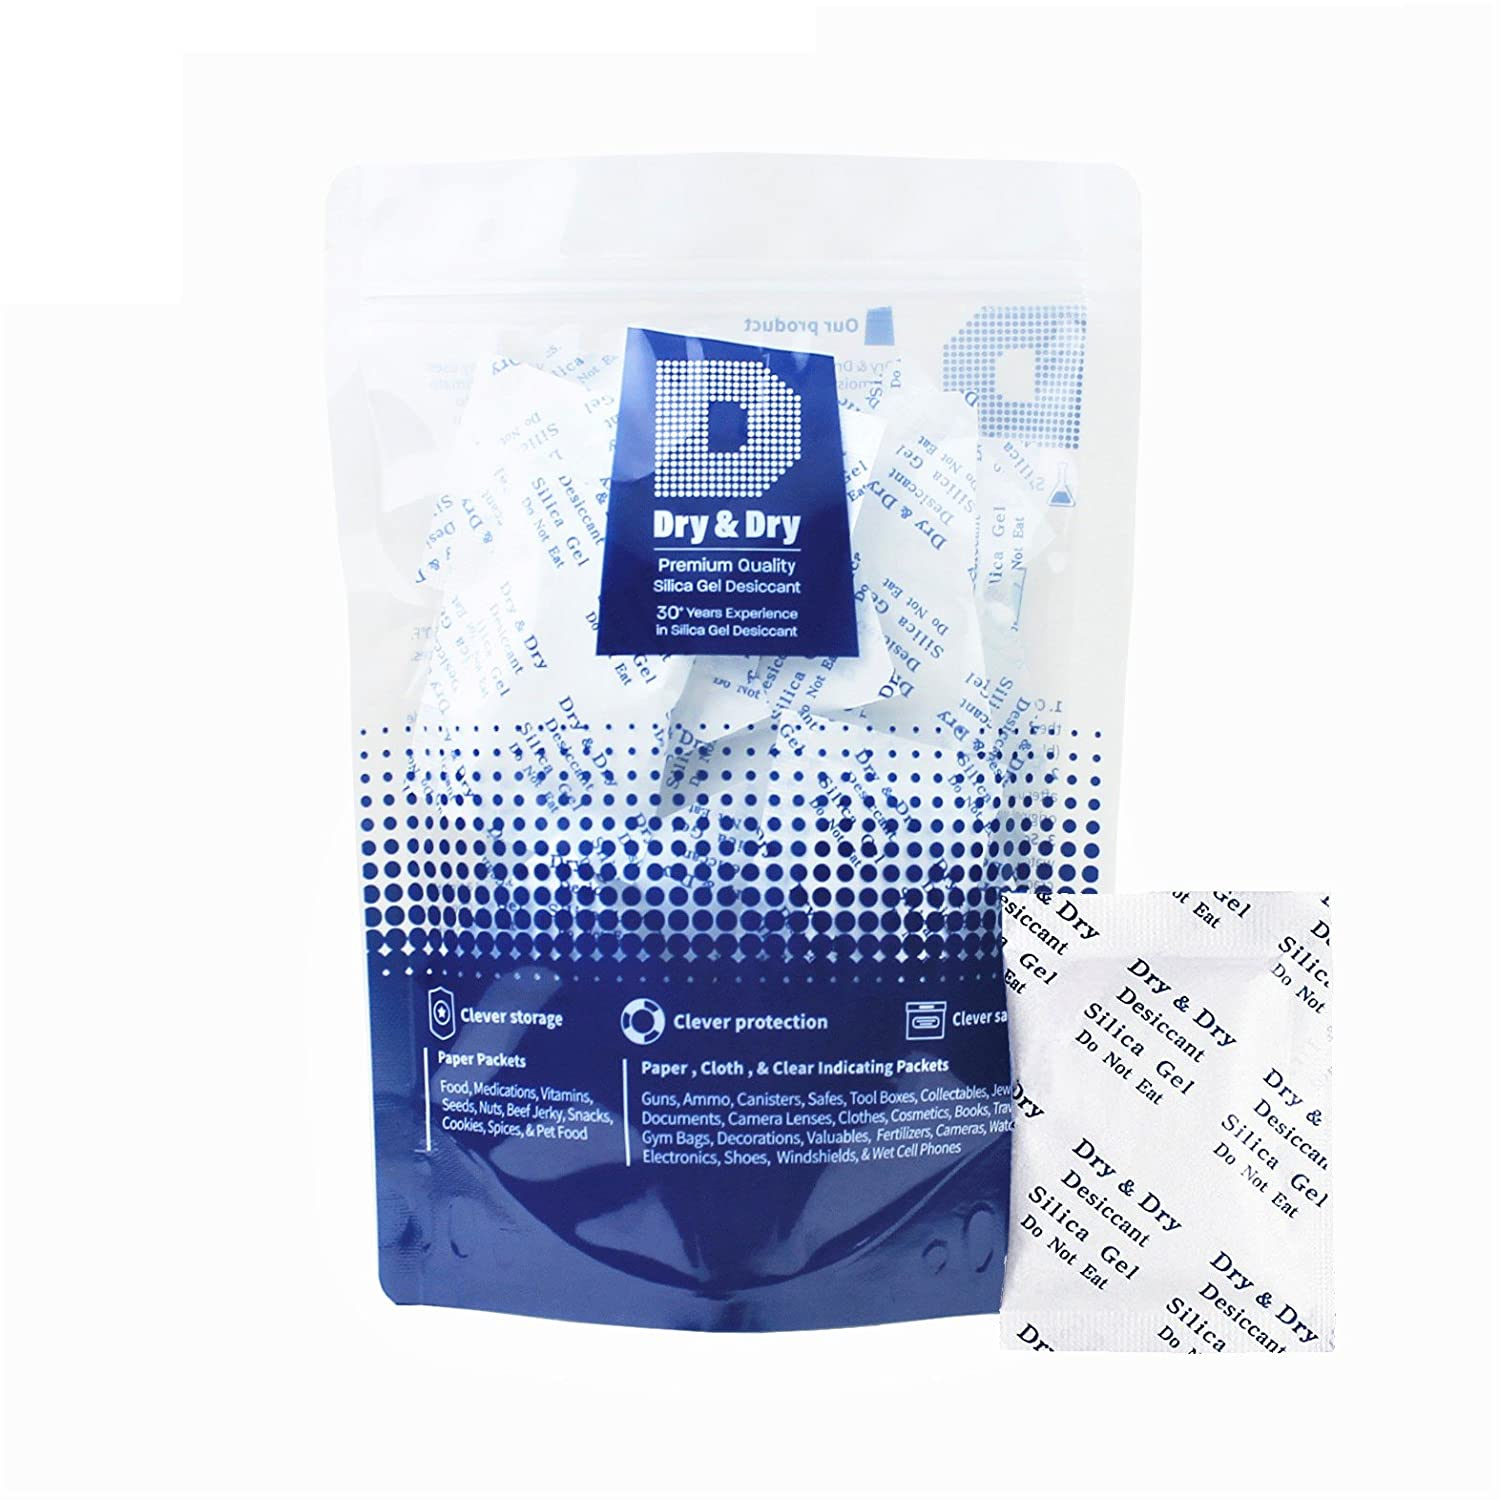
\includegraphics[scale=0.07]{silica.jpg}

\begin{flushleft}
    A packet of silica gels in the Nalgene bottle will be used as a dehumidifier, 
    to help maintain a humidity and moisture free enclosure of the electronic 
    components.
    \newline

    Online store link: \newline
    \footnotesize\url{https://www.amazon.com/Dry-Premium-Packets-Desiccant-Dehumidifiers/dp/B00DYKTS9C}

\end{flushleft}

\hypertarget{glue}{}
\subsubsection{Clear Silicone Sealant}

\hspace{2em}
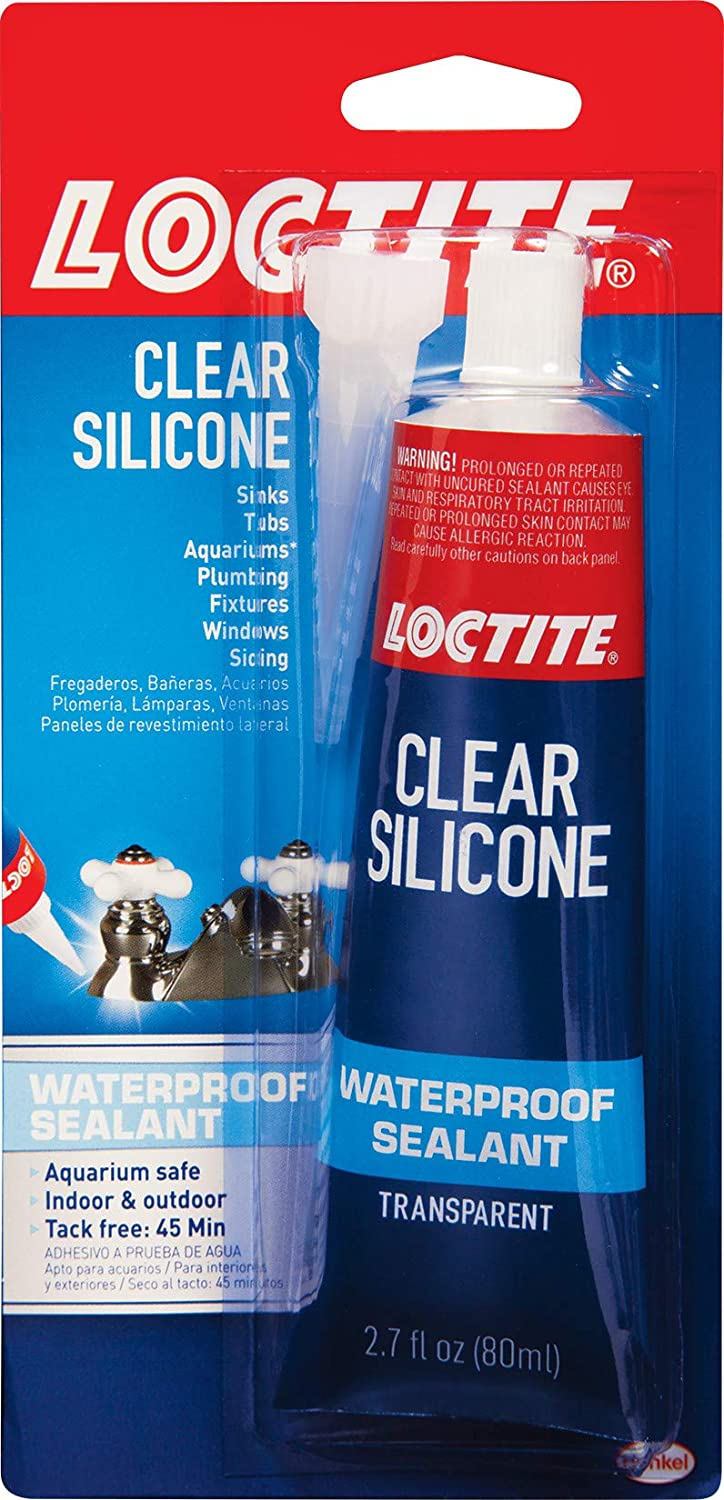
\includegraphics[scale=0.1]{silicone.jpg}

\begin{flushleft}
    A clear, waterproof silicone sealant to adhere and protect the exterior 
    sensors from water damage. It will also be used to adhere the jumper wires 
    in place and seal the two cables that will be protruding through the lid 
    of the Nalgene bottle.
    \newline

    Online store link: \newline
    \footnotesize\url{https://www.amazon.com/Loctite-Silicone-Waterproof-2-7-Ounce-908570/dp/B0002BBX3U}

\end{flushleft}

